\documentclass[a4paper, 11pt]{article}

%Comandos para configurar el idioma
\usepackage[spanish,activeacute]{babel}
\usepackage[utf8]{inputenc}
\usepackage[T1]{fontenc} %Necesario para el uso de las comillas latinas.

\usepackage{hyperref}
\hypersetup{
  pdftitle={Semana 2},
  pdfauthor={Alejandro García Montoro},
  unicode,
  plainpages=false,
  colorlinks,
  citecolor=black,
  filecolor=black,
  linkcolor=black,
  urlcolor=black,
}

%Paquetes matemáticos
\usepackage{amsmath,amsfonts,amsthm}
\usepackage[all]{xy} %Para diagramas
\usepackage{graphicx} %Inclusion imagenes
\usepackage{enumerate} %Personalización de enumeraciones
\usepackage{mathtools} %Para \coloneqq
\usepackage{tikz} %Dibujos
\usetikzlibrary{positioning} %Distancias y posicionamiento en tikz

%Tipografía escalable
\usepackage{lmodern}
%Legibilidad
\usepackage{microtype}

\title{Álgebra III \\ Semana 2}
\author{Alejandro García Montoro\\
    \href{mailto:agarciamontoro@correo.ugr.es}{agarciamontoro@correo.ugr.es}}
\date{\today}

\theoremstyle{definition}
\newtheorem{ejercicio}{Ejercicio}
\newtheorem*{solucion}{Solución}
\theoremstyle{remark}
\newtheorem{apartado}{Apartado}[ejercicio]

\begin{document}

  \maketitle

  \begin{ejercicio}
  \end{ejercicio}

  \begin{solucion}
      \begin{apartado}
          Sean $\alpha_1, \alpha_2, \alpha_3$ las raíces del polinomio \[p(X) = X^3 + aX^2 + bX +c\]
          Veamos qué relación hay entre las raíces y los coeficientes del polinomio. Por ser $\alpha_i$ las raíces de $p(X)$, sabemos que podemos escribir \[p(X) = (X-\alpha_1)(X-\alpha_2)(X-\alpha_3)\]
          Por tanto, llamando $e_i$ a los polinomios simétricos en los $\alpha_1, \alpha_2, \alpha_3$:
          \begin{align*}
             p(X) =& X^3 + (-\alpha_1 -\alpha_2 -\alpha_3)X^2 + (\alpha_1\alpha_2 + \alpha_1\alpha_3 + \alpha_2\alpha_3)X - \alpha_1\alpha_2\alpha_3 \implies \\
             e_1 \coloneqq& \alpha_1 + \alpha_2 + \alpha_3 = -a\\
             e_2 \coloneqq& \alpha_1\alpha_2 + \alpha_1\alpha_3 + \alpha_2\alpha_3 = b\\
             e_3 \coloneqq& \alpha_1\alpha_2\alpha_3 = -c
          \end{align*}

          Sea ahora $q(X) = X^3 + AX^2 + BX + C$ el polinomio cuyas raíces son $\alpha_1+\alpha_2, \alpha_1+\alpha_3$ y $\alpha_2+\alpha_3$. Vamos a expresar $A,B$ y $C$ en función de los coeficientes iniciales $a,b$ y $c$.

          Por los polinomios simétricos vistos anteriormente, tenemos lo siguiente:
          \begin{align*}
              -A =& (\alpha_1+\alpha_2) + (\alpha_1+\alpha_3) + (\alpha_2+\alpha_3) \\
              B =& (\alpha_1+\alpha_2)(\alpha_1+\alpha_3) + (\alpha_1+\alpha_2)(\alpha_2+\alpha_3) + (\alpha_1+\alpha_3)(\alpha_2+\alpha_3)\\
              -C =& (\alpha_1+\alpha_2)(\alpha_1+\alpha_3)(\alpha_2+\alpha_3)
          \end{align*}

          Trabajamos con cada ecuación por separado. Para el primer coeficiente:
          \[
          -A = 2(\alpha_1 + \alpha_2 + \alpha_3) = 2e_1 = -2a \implies \boxed{A = 2a}
          \]

          Para el segundo:
          \begin{align*}
              B &= 3(\alpha_1\alpha_2 + \alpha_1\alpha_3 + \alpha_2\alpha_3) + \alpha_1^2 + \alpha_2^2 + \alpha_3^2 = \\
                &= 3b + \alpha_1^2 + \alpha_2^2 + \alpha_3^2
          \end{align*}

          Para obtener una expresión cómoda de $m \coloneqq \alpha_1^2 + \alpha_2^2 + \alpha_3^2$, podemos hacer lo siguiente:
          \begin{align*}
          e_1^2 &= \alpha_1^2 + \alpha_2^2 + \alpha_3^2 + 2(\alpha_1\alpha_2+\alpha_1\alpha_3+\alpha_2\alpha_3) &\implies \\
          m - e_1^2 &= -2(\alpha_1\alpha_2+\alpha_1\alpha_3+\alpha_2\alpha_3) = -2e_2 &\implies \\
          m &= e_1^2 - 2e_2^2 = (-a)^2 -2b^2 = a^2 -2b^2
          \end{align*}

          Por tanto:
          \[
              B = 3b + m = 3b +a^2  -2b^2 \implies \boxed{B = a^2 -2b^2 + 3b}
          \]

          Para el último coeficiente, tenemos la expresión siguiente:
          \begin{align*}
              -C =& \alpha_1^2\alpha_2 + \alpha_1^2\alpha_3 + \\
                  & \alpha_2^2\alpha_1 + \alpha_2^2\alpha_3 + \\
                  & \alpha_3^3\alpha_1 + \alpha_3^2\alpha_2 + \\
                  & 2\alpha_1\alpha_2\alpha_3
          \end{align*}

          El último sumando es $2e_3$, así que trabajamos con todos los anteriores, a los que llamamos $r \coloneqq -C - 2e_3$.

          Haciendo cuentas, sabemos que $r-e_1e_2 = -3e_3$, así que concluimos que $r=e_1e_2 - 3e_3$

          Por tanto:
          \[
              -C -2e_3 = e_1e_2 - 3e_3 \implies C = -e_1e_2 + e_3 \implies \boxed{C = ab - c}
          \]

          Por tanto, el polinomio que buscamos es
          \[
          \boxed{q(X) = X^3 + 2aX^2 + (a^2 -2b^2 + 3b)X + ab -c}
          \]
      \end{apartado}

      \begin{apartado}
           Sea ahora $q(X) = X^3 + AX^2 + BX + C$ el polinomio cuyas raíces son $\alpha_1^2+\alpha_2^2, \alpha_1^2+\alpha_3^2$ y $\alpha_2^2+\alpha_3^2$. Como antes, vamos a expresar $A,B$ y $C$ en función de los coeficientes iniciales $a,b$ y $c$.

           La técnica es exactamente igual a la anterior, aunque ahora hay que hacer algo más de cuentas. Por eso, ayudarse de un programa de cálculo como Maxima es muy útil para seguir el algoritmo sin errores. Así se ha hecho en este ejercicio, así que no se dan con todo detalle las cuentas necesarias.

           En primer lugar, el coeficiente $A$ es directo. Teniendo en cuenta los valores de $e_i$ tenemos lo siguiente:
           \begin{align*}
               -A = (\alpha_1^2+\alpha_2^2) + (\alpha_1^2+\alpha_3^2) + (\alpha_2^2+\alpha_3^2) = 2(\alpha_1^2+\alpha_2^2+\alpha_3^2) = 2(e_1^2-2e_2)\\
               e_1 = -a; \;\;\; e_2 = b \;\;\; \implies \boxed{A = -2(a^2-2b)}
           \end{align*}

           Para el cálculo de $B$, se ha seguido la misma técnica que hasta ahora:
           \begin{enumerate}
               \item Expresión del coeficiente en función de las raíces usando su expresión en polinomios simétricos.
               \item Localización del monomio mayor ---en orden lexicográfico---.
               \item Cálculo del polinomio en los polinomios simétricos que elimina ese monomio:
               \begin{itemize}
                   \item Tomar los exponentes del monomio a eliminar; esto es, los $b_i$ del monomio $a\alpha_1^{b_1}\dots\alpha_n^{b_n}$.
                   \item Crear un polinomio en los polinomios simétricos como sigue:
                   \[ ae_1^{k_1} \dots e_n^{k_n} \]
                   donde $k_i = b_i - b_{i+1}$, tomando $b_{n+1} = 0$
               \end{itemize}
               \item Sustracción del polinomio anterior de la expresión inicial.
           \end{enumerate}

           Este algoritmo se ha realizado, como se ha indicado anteriormente, en Maxima. En la figura \ref{algoritmo} se ve este desarrollo. Por comodidad, en el código se han usado las letras $a,b,c$ en lugar de las $\alpha_1, \alpha_2, \alpha_3$. En el resto de este documento la notación sigue como hasta ahora.

           \begin{figure}[ht!]
               \centering
               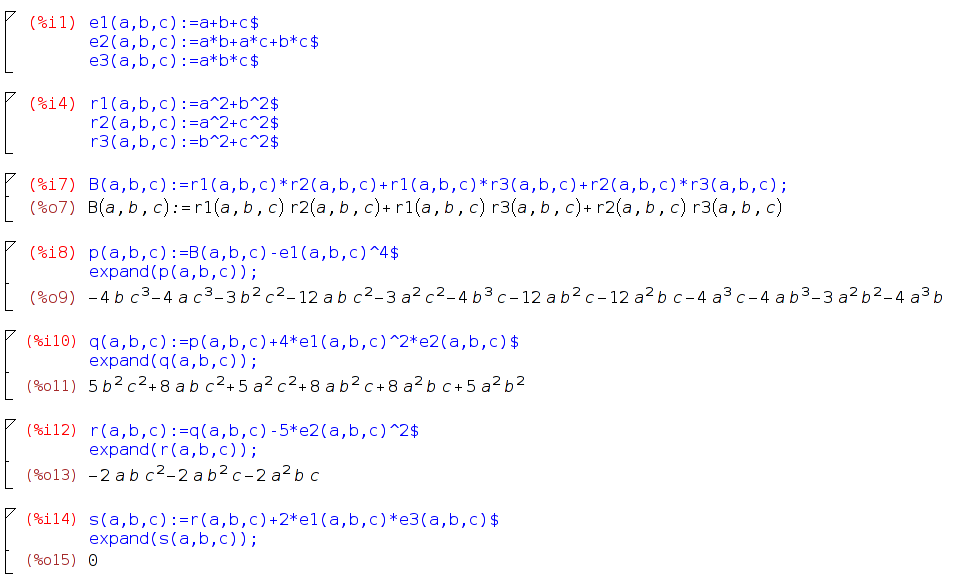
\includegraphics[width=130mm]{IMG/S02-01.png}
               \caption{Cálculo en Maxima del coeficiente $B$. \label{algoritmo}}
           \end{figure}

           Por tanto, como tenemos que $B = e_1^4-4e_1^2e_2+5e_2^2-2e_1e_3$, concluimos que el valor de $B$ es:
           \[
           \boxed{B = a^4 - 4a^2b + 5b^2 - 2ac}
           \]

           El cálculo de $C$ se ha hecho de la misma forma, como se ve en la figura \ref{algoritmo2}.

           \begin{figure}[ht!]
               \centering
               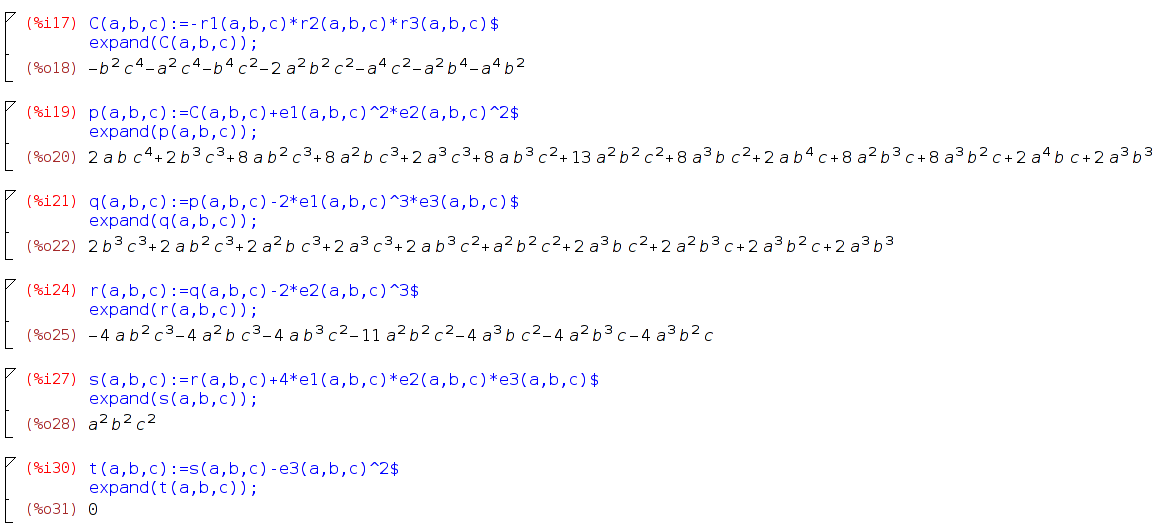
\includegraphics[width=140mm]{IMG/S02-02.png}
               \caption{Cálculo en Maxima del coeficiente $C$. \label{algoritmo2}}
           \end{figure}

           Así, concluimos que
           \[
           \boxed{C = -a^2b^2 + 2a^3c + 2b^3 -4abc +c^2}
           \]

           Finalmente, podemos definir explícitamente el polinomio $q(X)$ como sigue:
           \[
           \boxed{q(X) = X^3 - 2(a^2-2b)X^2 + (a^4 - 4a^2b + 5b^2 - 2ac)X + 2a^3c - a^2b^2 + 2b^3 -4abc +c^2}
           \]
      \end{apartado}
  \end{solucion}

  \begin{ejercicio}
  \end{ejercicio}

  \begin{solucion}
      Sean $a,b$ y $c$ los números que cumplen
      \begin{align*}
          a+b+c &= -3 \\
          a^2+b^2+c^3 &= 6 \\
          a^3+b^3+c^3 &= -3
      \end{align*}

      Por el estudio de polinomios simétricos, sabemos que $a,b,c$ son las raíces del polinomio siguiente:
      \[
      p(X) = X^3 -e_1 X^2 + e_2 X - e_3 = X^3 - (a+b+c) X^2 + (ab+ac+bc) X - abc
      \]

      Donde, como se aprecia, los $e_i$ son los polinomios simétricos en las variables $a,b,c$. Por tanto, podemos hacer un estudio del polinomio cuyas raíces cumplen el sistema que nos da el enunciado. Así, sus ecuaciones las podemos expresar en función de los polinomios simétricos tal y como sigue:
      \begin{align*}
          e_1 &= -3 \\
          e_1^2-2e_2 &= 6 \\
          e_1^3 -3e_1e_2 +3e_3 &= -3
      \end{align*}

      De aquí es directo deducir los valores de los $e_i$:
      \begin{align*}
          e_1 &= -3 \\
          e_2 &= \frac{3}{2} \\
          e_3 &= \frac{7}{2}
      \end{align*}

      Por tanto, ya tenemos la respuesta a la pregunta: la única terna de números $a,b,c$ ---salvo orden--- cuya suma vale $-3$, cuya suma de cuadrados vale $6$ y cuya suma de cubos vale $-3$ es la que está formada por las tres raíces del polinomio siguiente:

      \[
      \boxed{p(X) = X^3 +3X^2 + \frac{3}{2}X - \frac{7}{2}}
      \]
  \end{solucion}

  \begin{ejercicio}
  \end{ejercicio}

  \begin{solucion}
      Sean $\alpha_1, \alpha_2, \alpha_3$ las raíces del polinomio $p(X)=X^3+X^2-X-k$. Sabemos que verifican la relación

      \begin{equation} \label{rel}
          \alpha_1^2-\alpha_2^2+\alpha_3^3 = 0
      \end{equation}

      De la definición del polinomio, teniendo en cuenta el estudio de polinomios simétricos que venimos haciendo, sabemos lo siguiente:
      \begin{align*}
          e_1 &= \alpha_1+\alpha_2+\alpha_3 &=& -1 \\
          e_2 &= \alpha_1\alpha_2 + \alpha_1\alpha_3 + \alpha_2\alpha_3 &=& -1 \\
          e_3 &= \alpha_1\alpha_2\alpha_3 &=& k
      \end{align*}

      Por otro lado, de la relación \ref{rel}, deducimos lo siguiente:
      \begin{align*}
          \alpha_1^2+\alpha_2^2+\alpha_3^2 - 2\alpha_2^2 = 0
      \end{align*}

      Por estudios anteriores, sabemos que esto lo podemos expresar como sigue:
      \begin{equation} \label{alpha2}
        e_1^2-2e_2 - 2\alpha_2^2 = 0 \implies \boxed{\alpha_2 = \pm\sqrt{\frac{3}{2}}}
      \end{equation}

      Además, de los valores de $e_1$ y $e_2$, usando la igualdad vista en \ref{alpha2} podemos sacar más relaciones interesantes:
      \begin{align}
          e_2 = \alpha_1\alpha_2 + \alpha_1\alpha_3 + \alpha_2\alpha_3 \implies \boxed{-1 = \pm\sqrt{\frac{3}{2}}(\alpha_1+\alpha_3)+\alpha_1\alpha_3} \label{total}\\
          e_1 = \alpha_1 + \alpha_2 + \alpha_3 \implies \boxed{\alpha_1 + \alpha_3 = -1 \overline{+}\sqrt{\frac{3}{2}}} \label{suma}\\
          e_3 = \alpha_1\alpha_2\alpha_3 \implies \boxed{\alpha_1\alpha_3 = \pm\sqrt{\frac{2}{3}}k}\label{producto}
      \end{align}

      Sustituyendo \ref{suma} y \ref{producto} en \ref{total}, tenemos una relación de la que podemos despejar $k$:
      \begin{align*}
          -1 = \pm\sqrt{\frac{3}{2}}(-1\overline{+}\sqrt{\frac{3}{2}})\pm\sqrt{\frac{2}{3}}k &\implies \\
          \pm\sqrt{\frac{2}{3}}k = -1 \overline{+}\sqrt{\frac{3}{2}}(-1\overline{+}\sqrt{\frac{3}{2}}) &\implies \\
          \pm\sqrt{\frac{2}{3}}k = -1 \pm\sqrt{\frac{3}{2}} + \frac{3}{2} &\implies \\
          k = \pm\sqrt{\frac{3}{2}}(-1 \pm\sqrt{\frac{3}{2}} + \frac{3}{2}) &\implies \\
          k = \overline{+}\sqrt{\frac{3}{2}} + \frac{3}{2} \pm\frac{3}{2}\sqrt{\frac{3}{2}} &\implies \\
          k = \pm\sqrt{\frac{3}{2}}(\frac{3}{2}-1) + \frac{3}{2} &\implies \\
          \boxed{k = \frac{3}{2} \pm \frac{1}{2}\sqrt{\frac{3}{2}}} &
      \end{align*}



  \end{solucion}

\end{document}
